\documentclass{article}

\usepackage[T1]{fontenc}    %Schriftart des Dokumentes
\usepackage[ngerman]{babel} %Dokumentensprache, hier Deutsch
\usepackage{amsmath, amssymb, stmaryrd} %mathematische Schriftzeichen
\usepackage{graphicx} %Einfügen von Grafiken
\usepackage{wrapfig}
\usepackage{bm}

\setlength{\parindent}{0pt} %Einrückung von Absätzen auf null gesetzt
\setlength{\parskip}{10pt} %Abstand zischen Absätzen auf 10pt gesetzt

\title{Versuch 42: Spezifische Wärmekapazität fester Körper}
\author{Matthias Kuntz}
\date{15.09.2023}

\begin{document}

\maketitle

%-------------------------EINLEITUNG-------------------------
\section{Einleitung}

In diesem Versuch sollen auf zwei verschiedenen Wegen die Wärmekapazitäten von Graphit, Aluminium und Blei bestimmt werden. Im ersten Teil wird untersucht, wie sich die Temperatur entwickelt, wenn man heißes Wasser in ein Kalorimeter füllt und dieses abkühlen lässt, um den Wasserwert des Kalorimeters zu befüllen. Danach werden heiße Porbekörper bestehend aus den drei Materialien nacheinander in Wasser eingetaucht und die Temperaturentwicklung untersucht. Daraufhin untersuchen wir, wieviel einer festen Menge flüssigen Stickstoffs verdampft, wenn Probekörper in diesen eingelassen werden. Zum Schluss finden dann noch Vergleiche mit dem Dulong-Petit-Gesetzt und der Debyetheorie statt. 

\subsection{Physikalische Grundlagen}

Wird einem Körper eine Wärmemenge $Q$ zugeführt, so ist die Temperaturänderung $\Delta T$ abhängig von der sogenannten Wärmekapazität $C$ des Körpers. Findet dabei kein Phasenübergang statt gilt:

\begin{equation}
    C=\frac{Q}{\Delta T}
\end{equation}

Allgemein ist diese Größe auch masseabhängig, weshalb man die spezifische Wärmekapazität $c$ über die Masse $m$ sowie die molare Wärmekapazität (Molwärme) $c_m$ über die Molare Masse $M$ definiert:

\begin{equation}
    \begin{split}
        c &= \frac{C}{m} = \frac{Q}{m \Delta T} \\
        c_m &= M c = \frac{MQ}{m \Delta T}
    \end{split}
\end{equation}

Berühren sich zwei Körper unterschiedlicher Temperaturen so findet ein Temperaturausgleich über den Austausch von Wärmemengen statt. Haben die beiden Körper jeweils die Temperaturen $T_1$ und $T_2$, sei hier $T_1 > T_2$, so stellt sich die Mischtemperatur $\overline{T}$ ein und die vom Körper 1 abgegebene Wärmemenge $Q_1$ ist gleich der vom Körper 2 aufgenommen Wärmemenge $Q_2$. Bei uns sind im ersten Versuchsteil Körper 1 die Probemassen aus Graphit, Aluminium und Blei (Index $x$) und Körper 2 sind das Wasser (Index $W$) sowie das Kalorimeter, in dem sich das Wasser befindet. Somit ergibt sich für uns:

\begin{equation}
    \begin{split}
        Q_1 &= m_x c_x (T_1 - \overline{T}) \\
        Q_2 &= (m_W c_W + W)(\overline{T} - T_2)
    \end{split}
\end{equation}

Die Größe W bezeichnet hier den sogenannten Wasserwert, der die Wärmekapazität des Kalorimeters darstellt. Aus diesen Beiden Formeln lässt sich die gesuchte spezifische Wärmekapazität berechnen. Aus $Q_1 = Q_2$ folt dann:

\begin{equation}
    c_x = \frac{(c_W m_W + W) (\overline{T} - T_2)}{m_x (T_1 - \overline{T})}
\end{equation}

Die spezifische Wärmekapazität von Wasser beträgt im Bereich von 15$^\circ$C bis 65$^\circ$C etwa $c_W = (4,186 \pm 0,004) \frac{\text{J}}{\text{g} \cdot \text{K}}$.

Wird ein Probekörper in flüssigen Stickstoff ($T_2 = -195,8^\circ$C) getaucht, so verdampft ein Teil des Stickstoffs. Aus der Verdampfungswärme $Q_V$ und der verdampften Menge $m_V$ kann zunächst die abgegebene Wärme $Q$ des Probekörpers und schließlich die spezifische Wärmekapazität berechnet werden:

\begin{equation}
    Q = Q_V m_V = m_x c_x (T_1 - T_2)
\end{equation}

\newpage

\subsection{Versuchsaufbau}

Eine Skizze des Versuchsaufbaus ist auf der nächsten Seite im Messprotokoll zu sehen. 

Zunächst werden alle Massen der insgesamt sechs Probekörper, zwei pro Material, bestimmt. Danach beginnt der erste Versuchsteil, bei dem das Kalorimeter mit warmem Wasser befüllt und der Temperaturabfall beobachtet wird. Dann werden nacheinander die großen Probekörper in kochendem Wasser erhitzt und in das Wasserbad im Kalorimeter gelassen. Dabei wird vor und nach Einlass des Probekörpers immer wieder die Temperatur aufgezeichnet und das Kalorimeter wird zunächt leer sowie immer vor jedem Probekörper gewogen.

Anschließend wird ein Dewar mit flüssigem Stickstoff befüllt und es werden nacheinander die drei kleinen Probekörper hineingehalten. Dabei wird immer vorher und nachher das Gewicht des Dewars gemessen. Aus der Differenz von den beiden Massen erhält man die Masse des verdampften Stickstoffs.

%---------------VERSUCHSPROTOKOLL MIT MESSDATEN---------------
\newpage

\section{Versuchsprotokoll mit Messdaten}

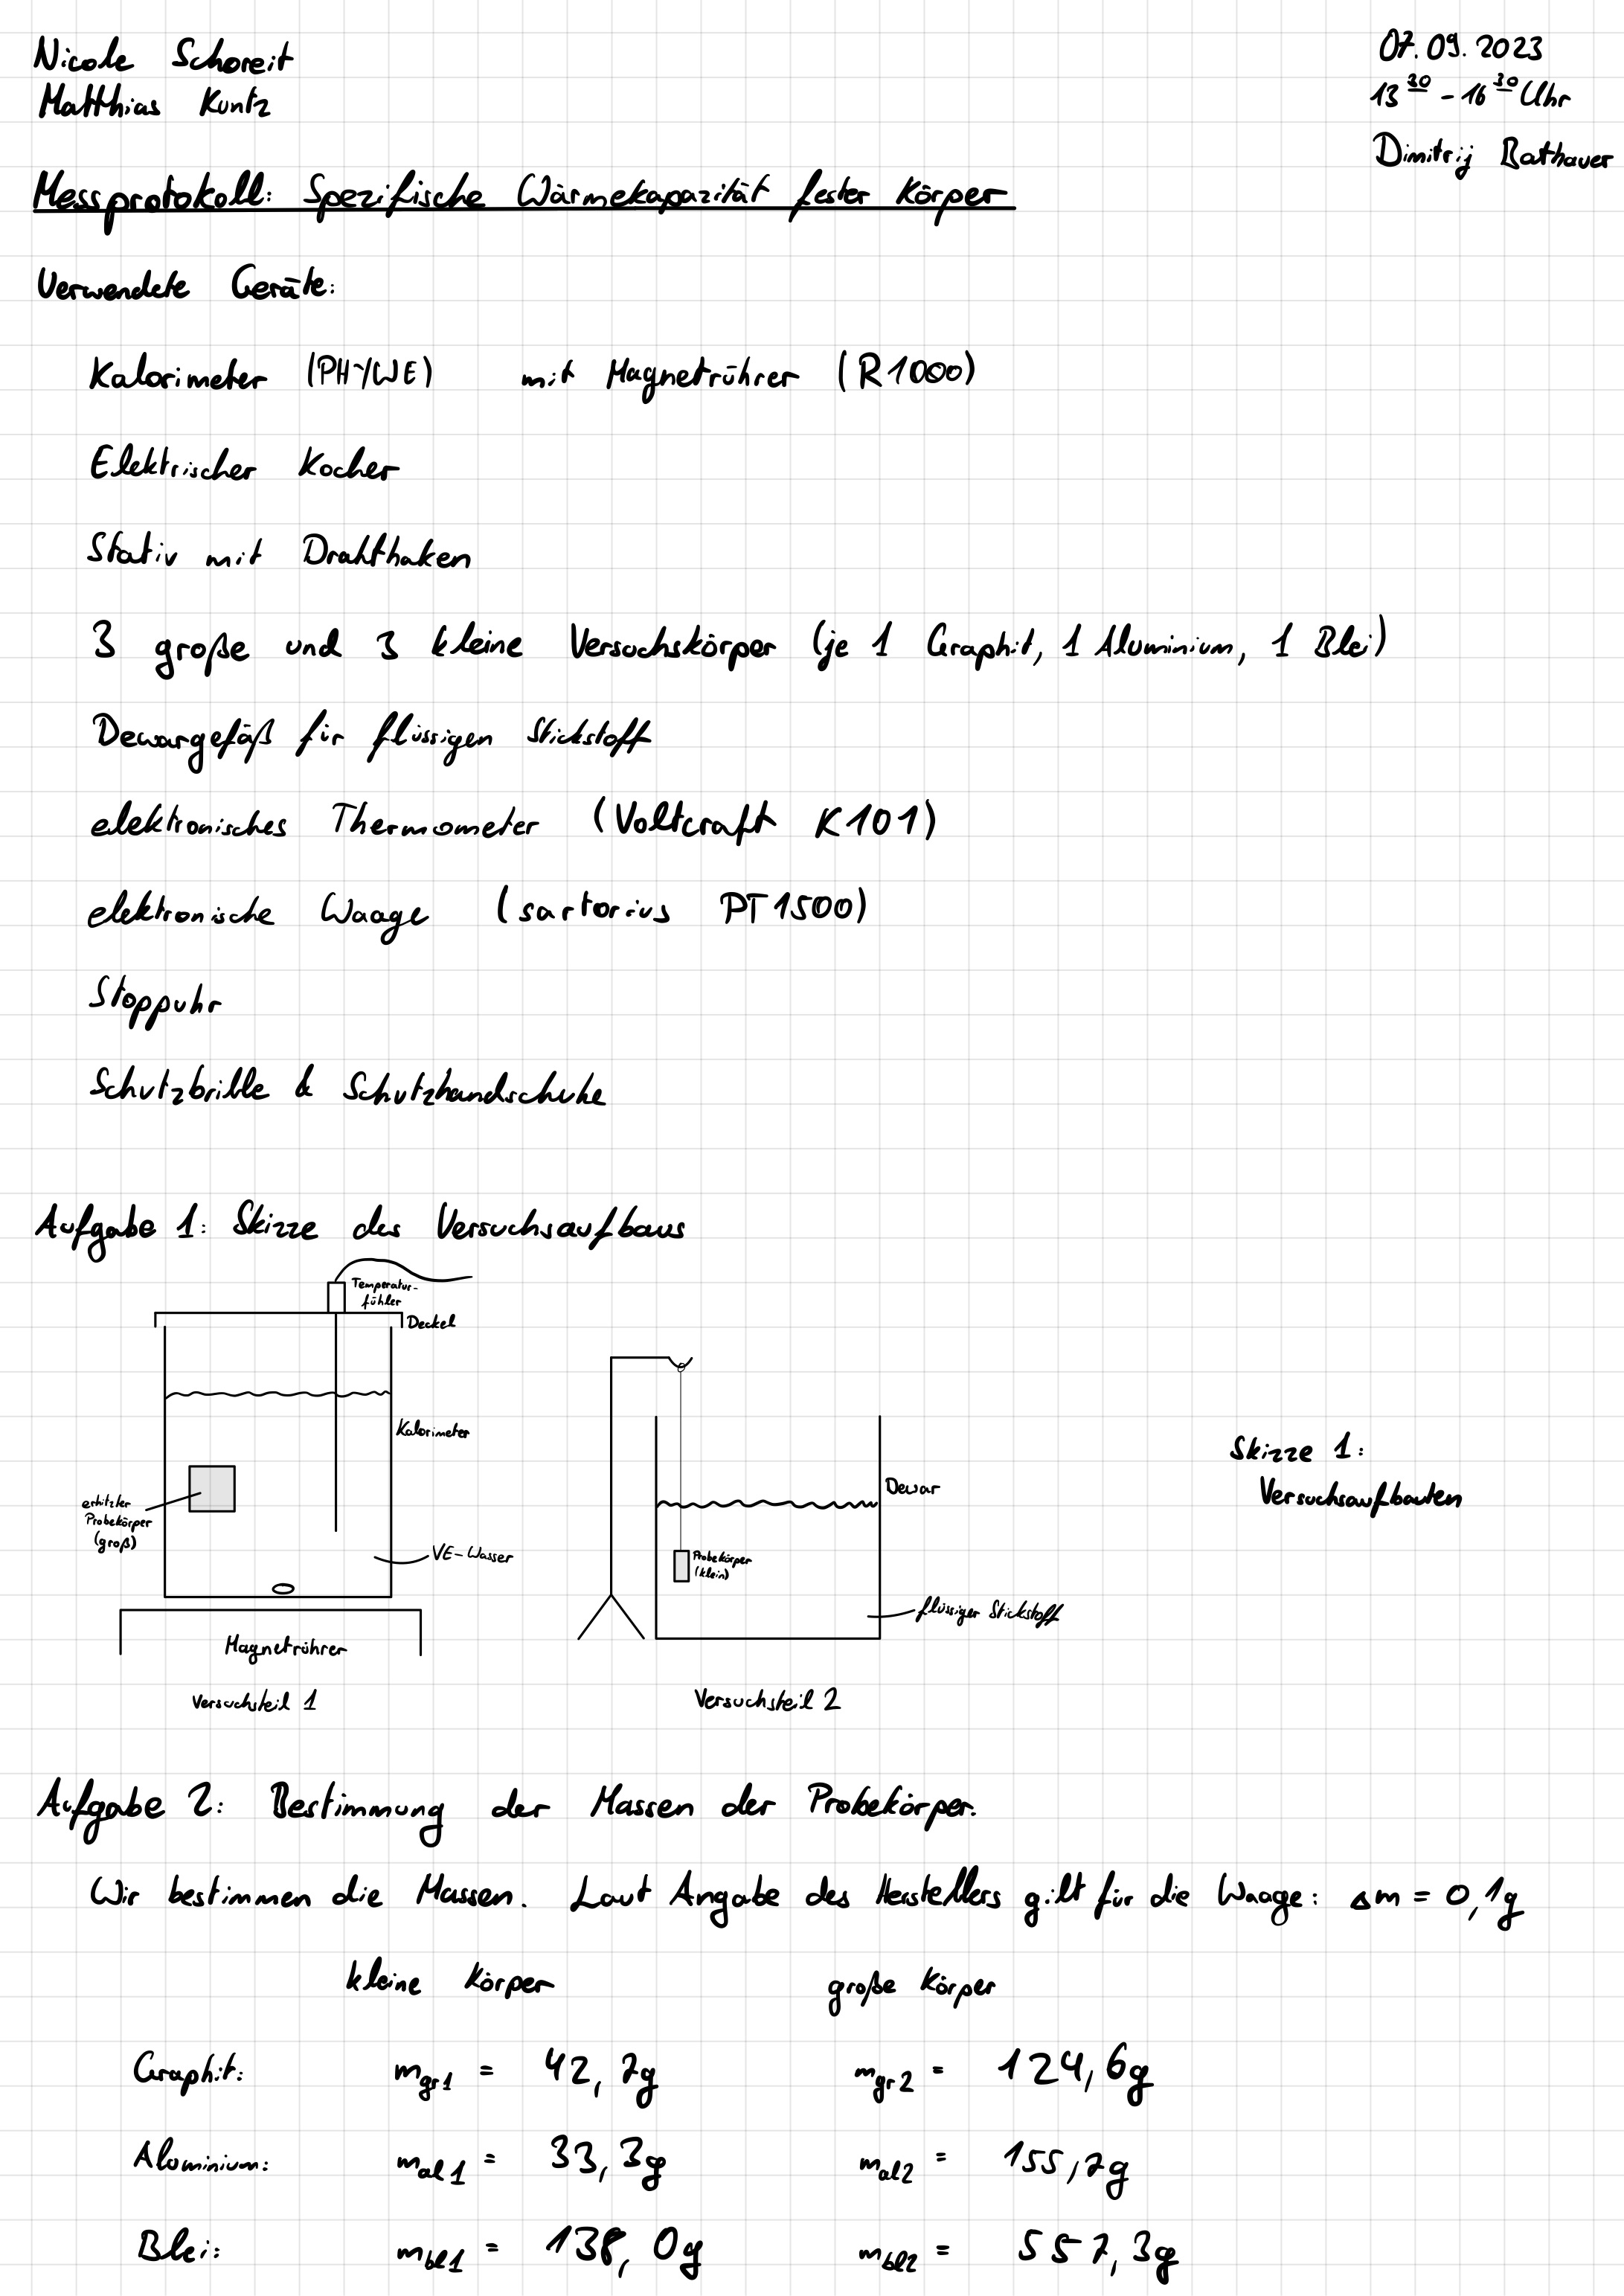
\includegraphics[width=\textwidth]{graphics/mess1.jpg}
\newpage
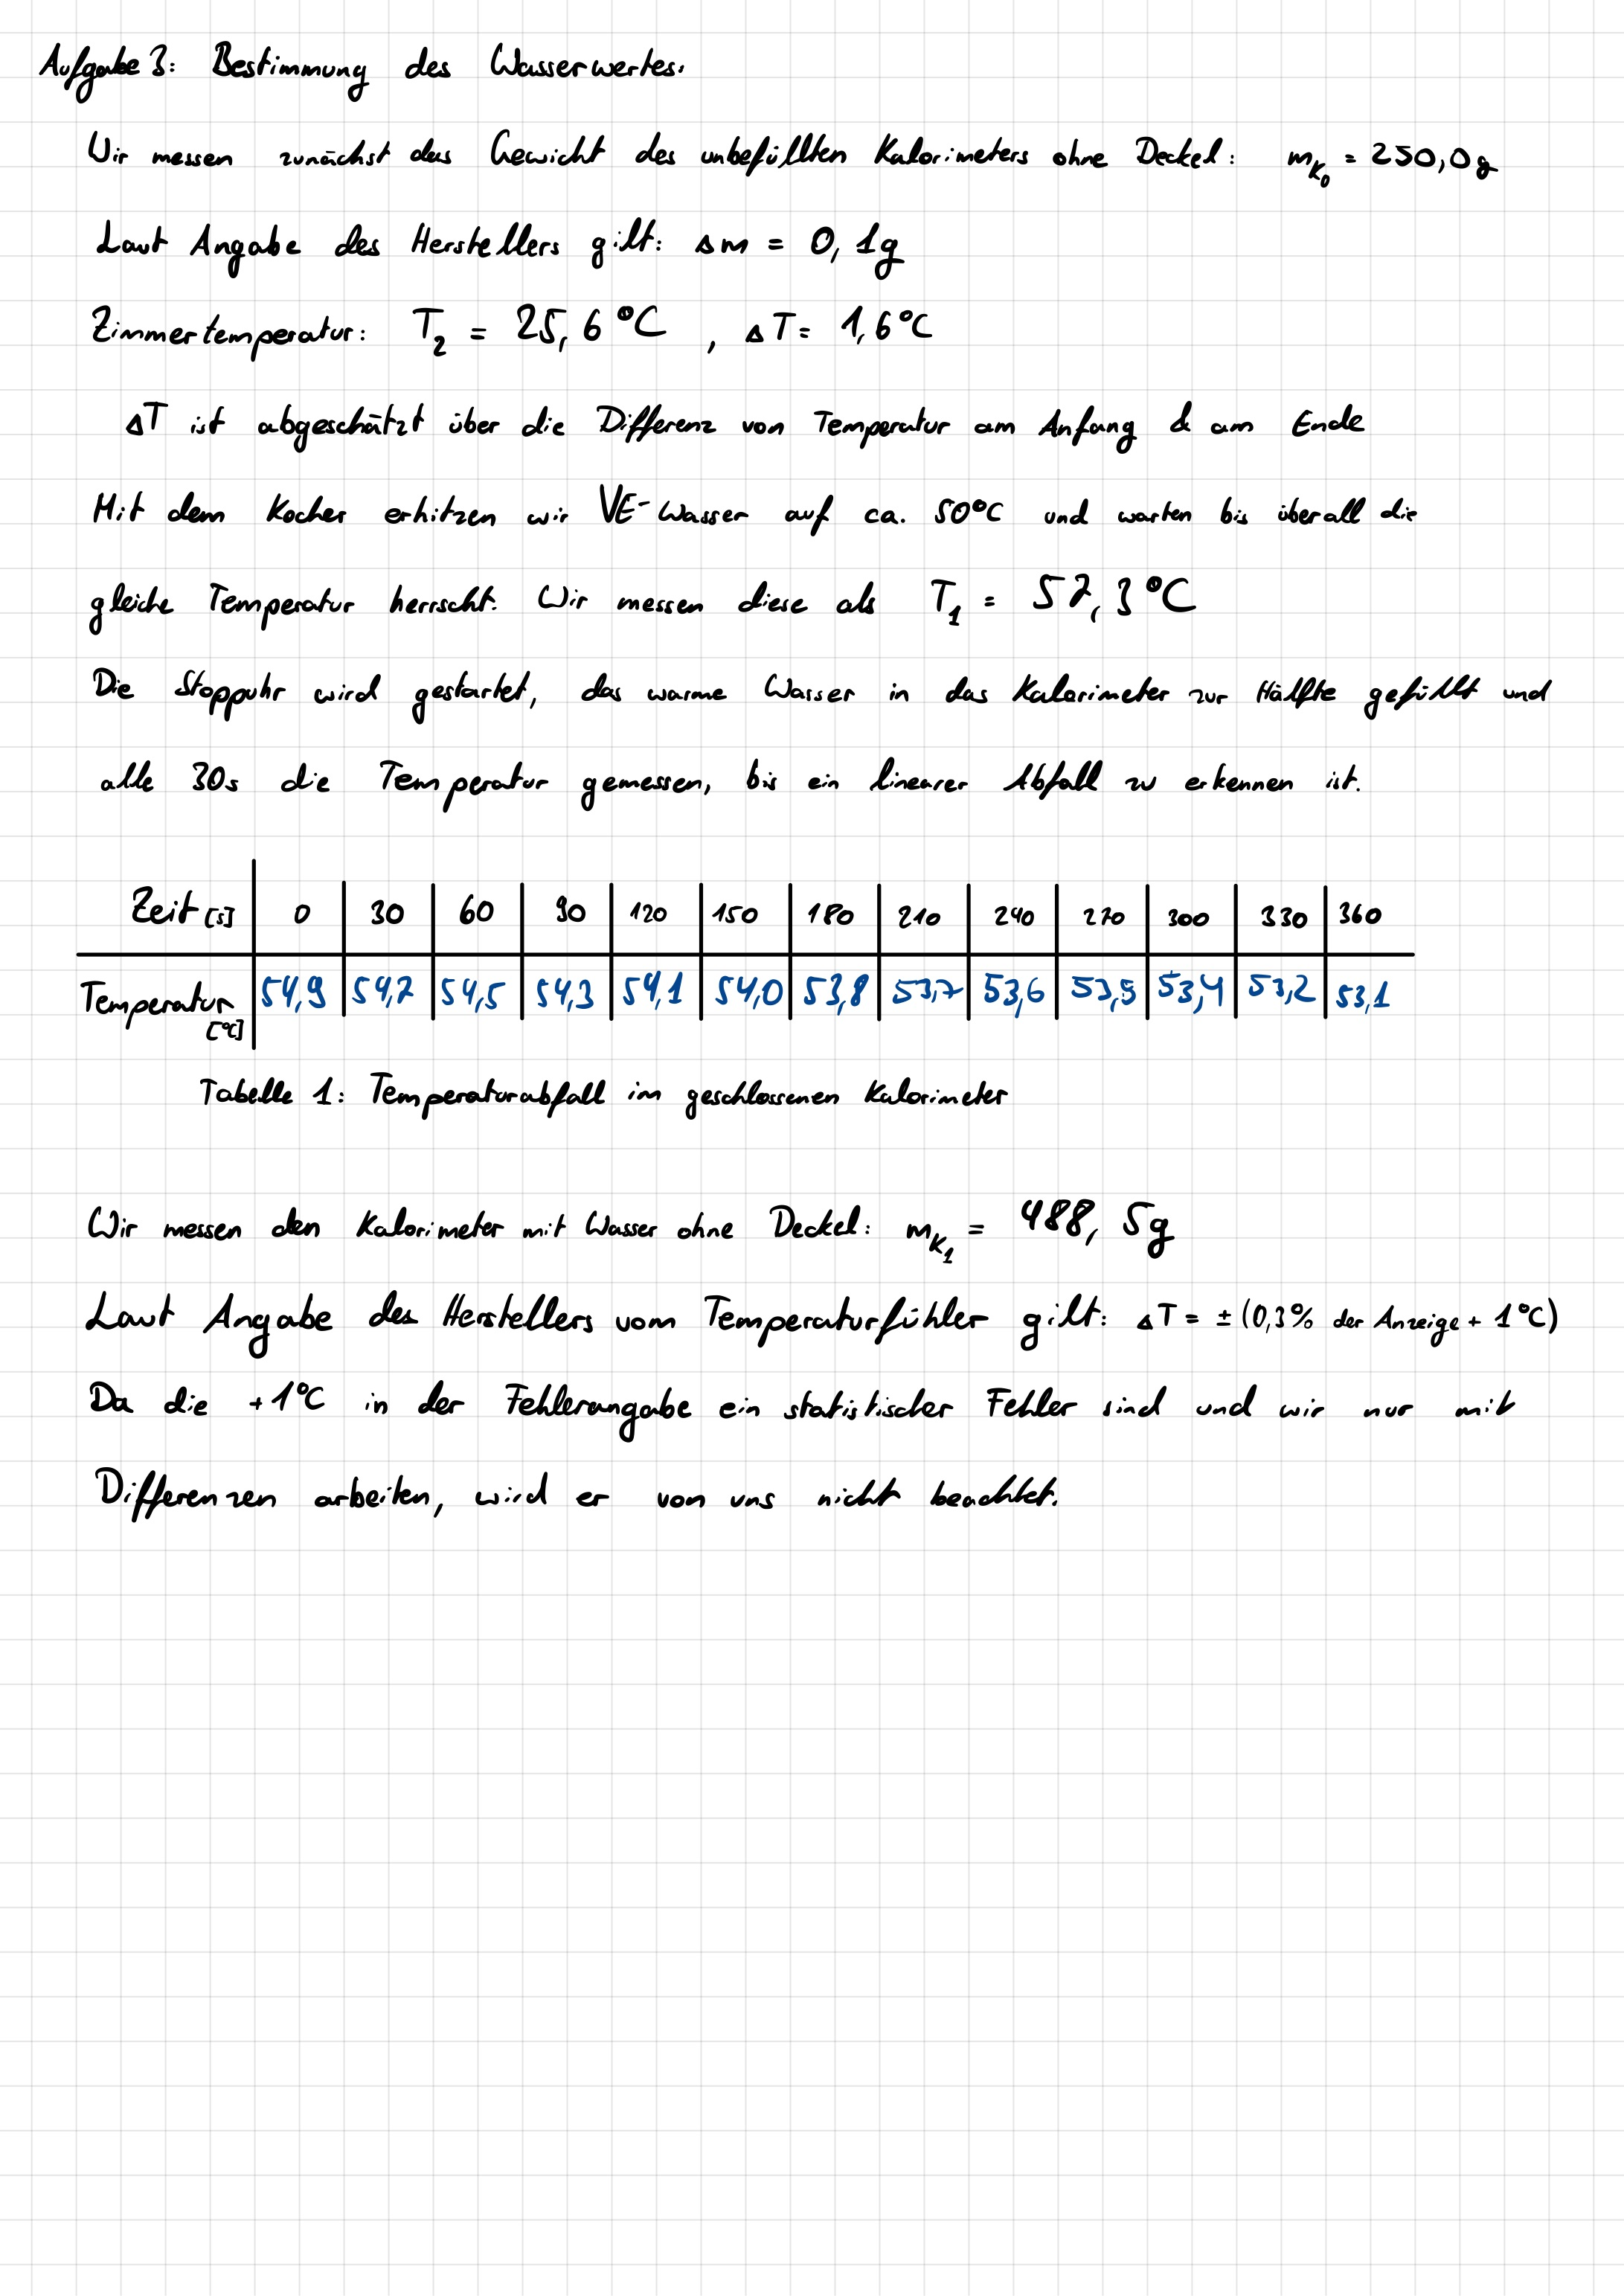
\includegraphics[width=\textwidth]{graphics/mess2.jpg}
\newpage
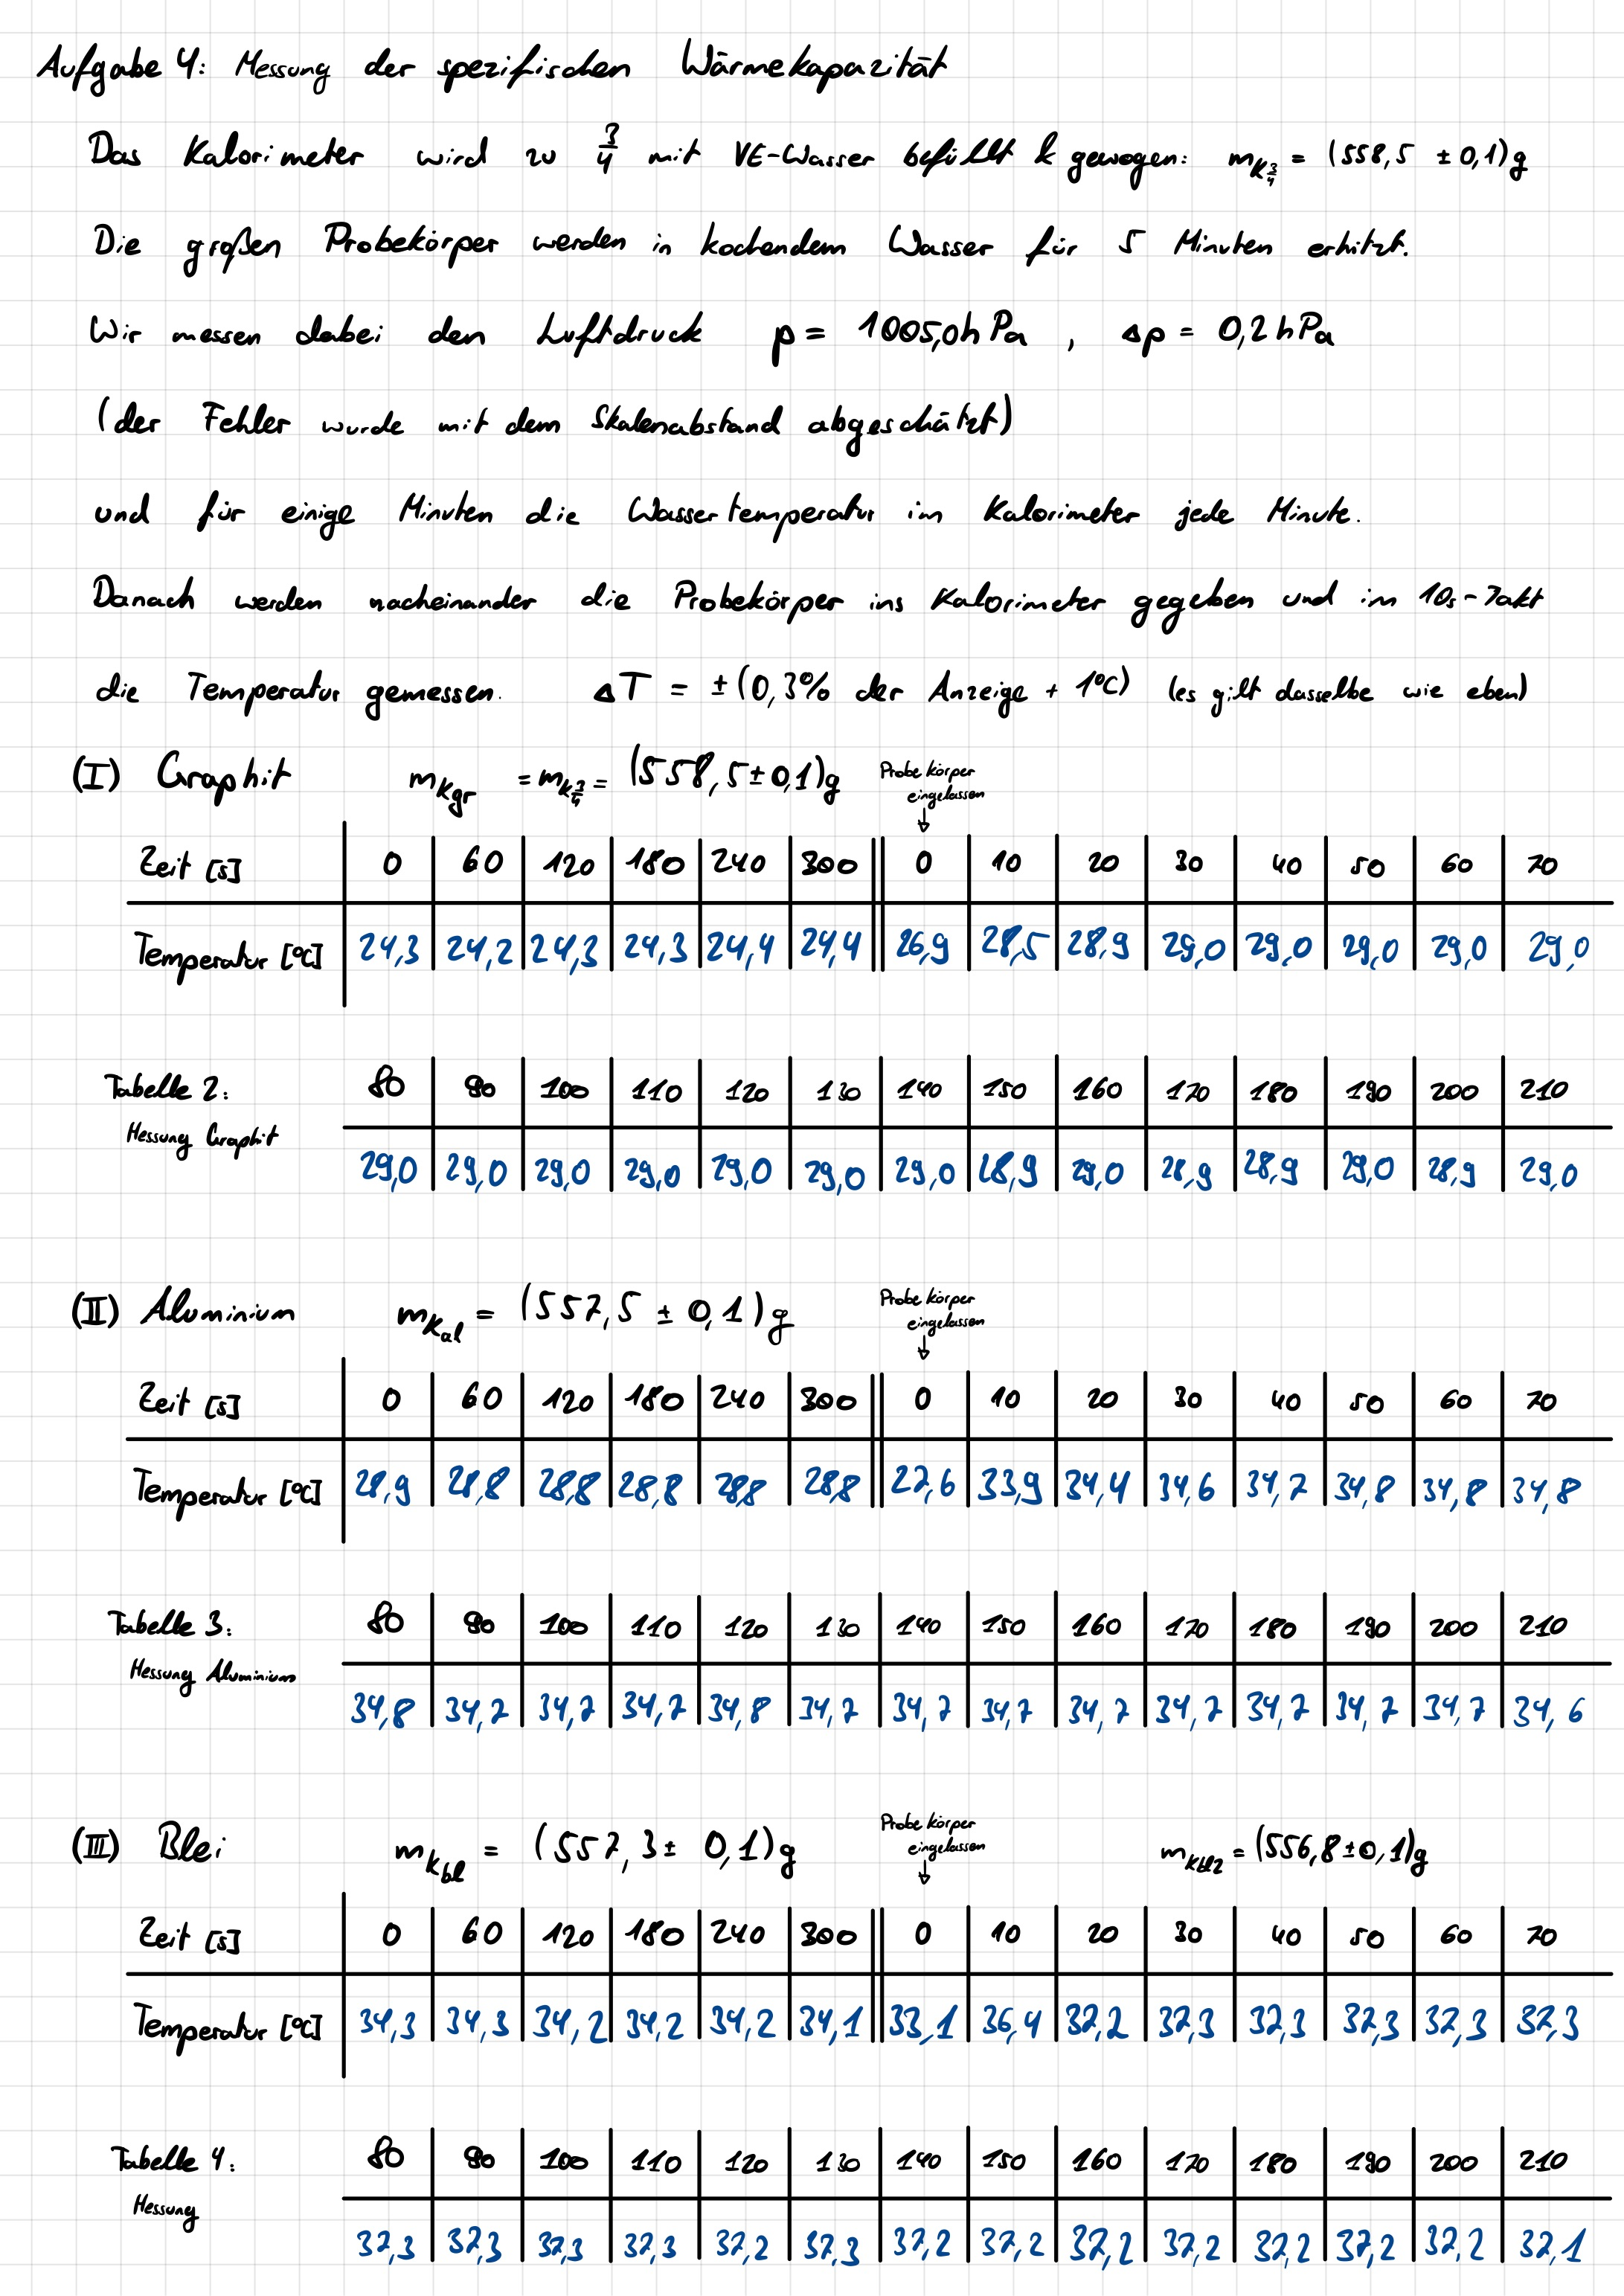
\includegraphics[width=\textwidth]{graphics/mess3.jpg}
\newpage
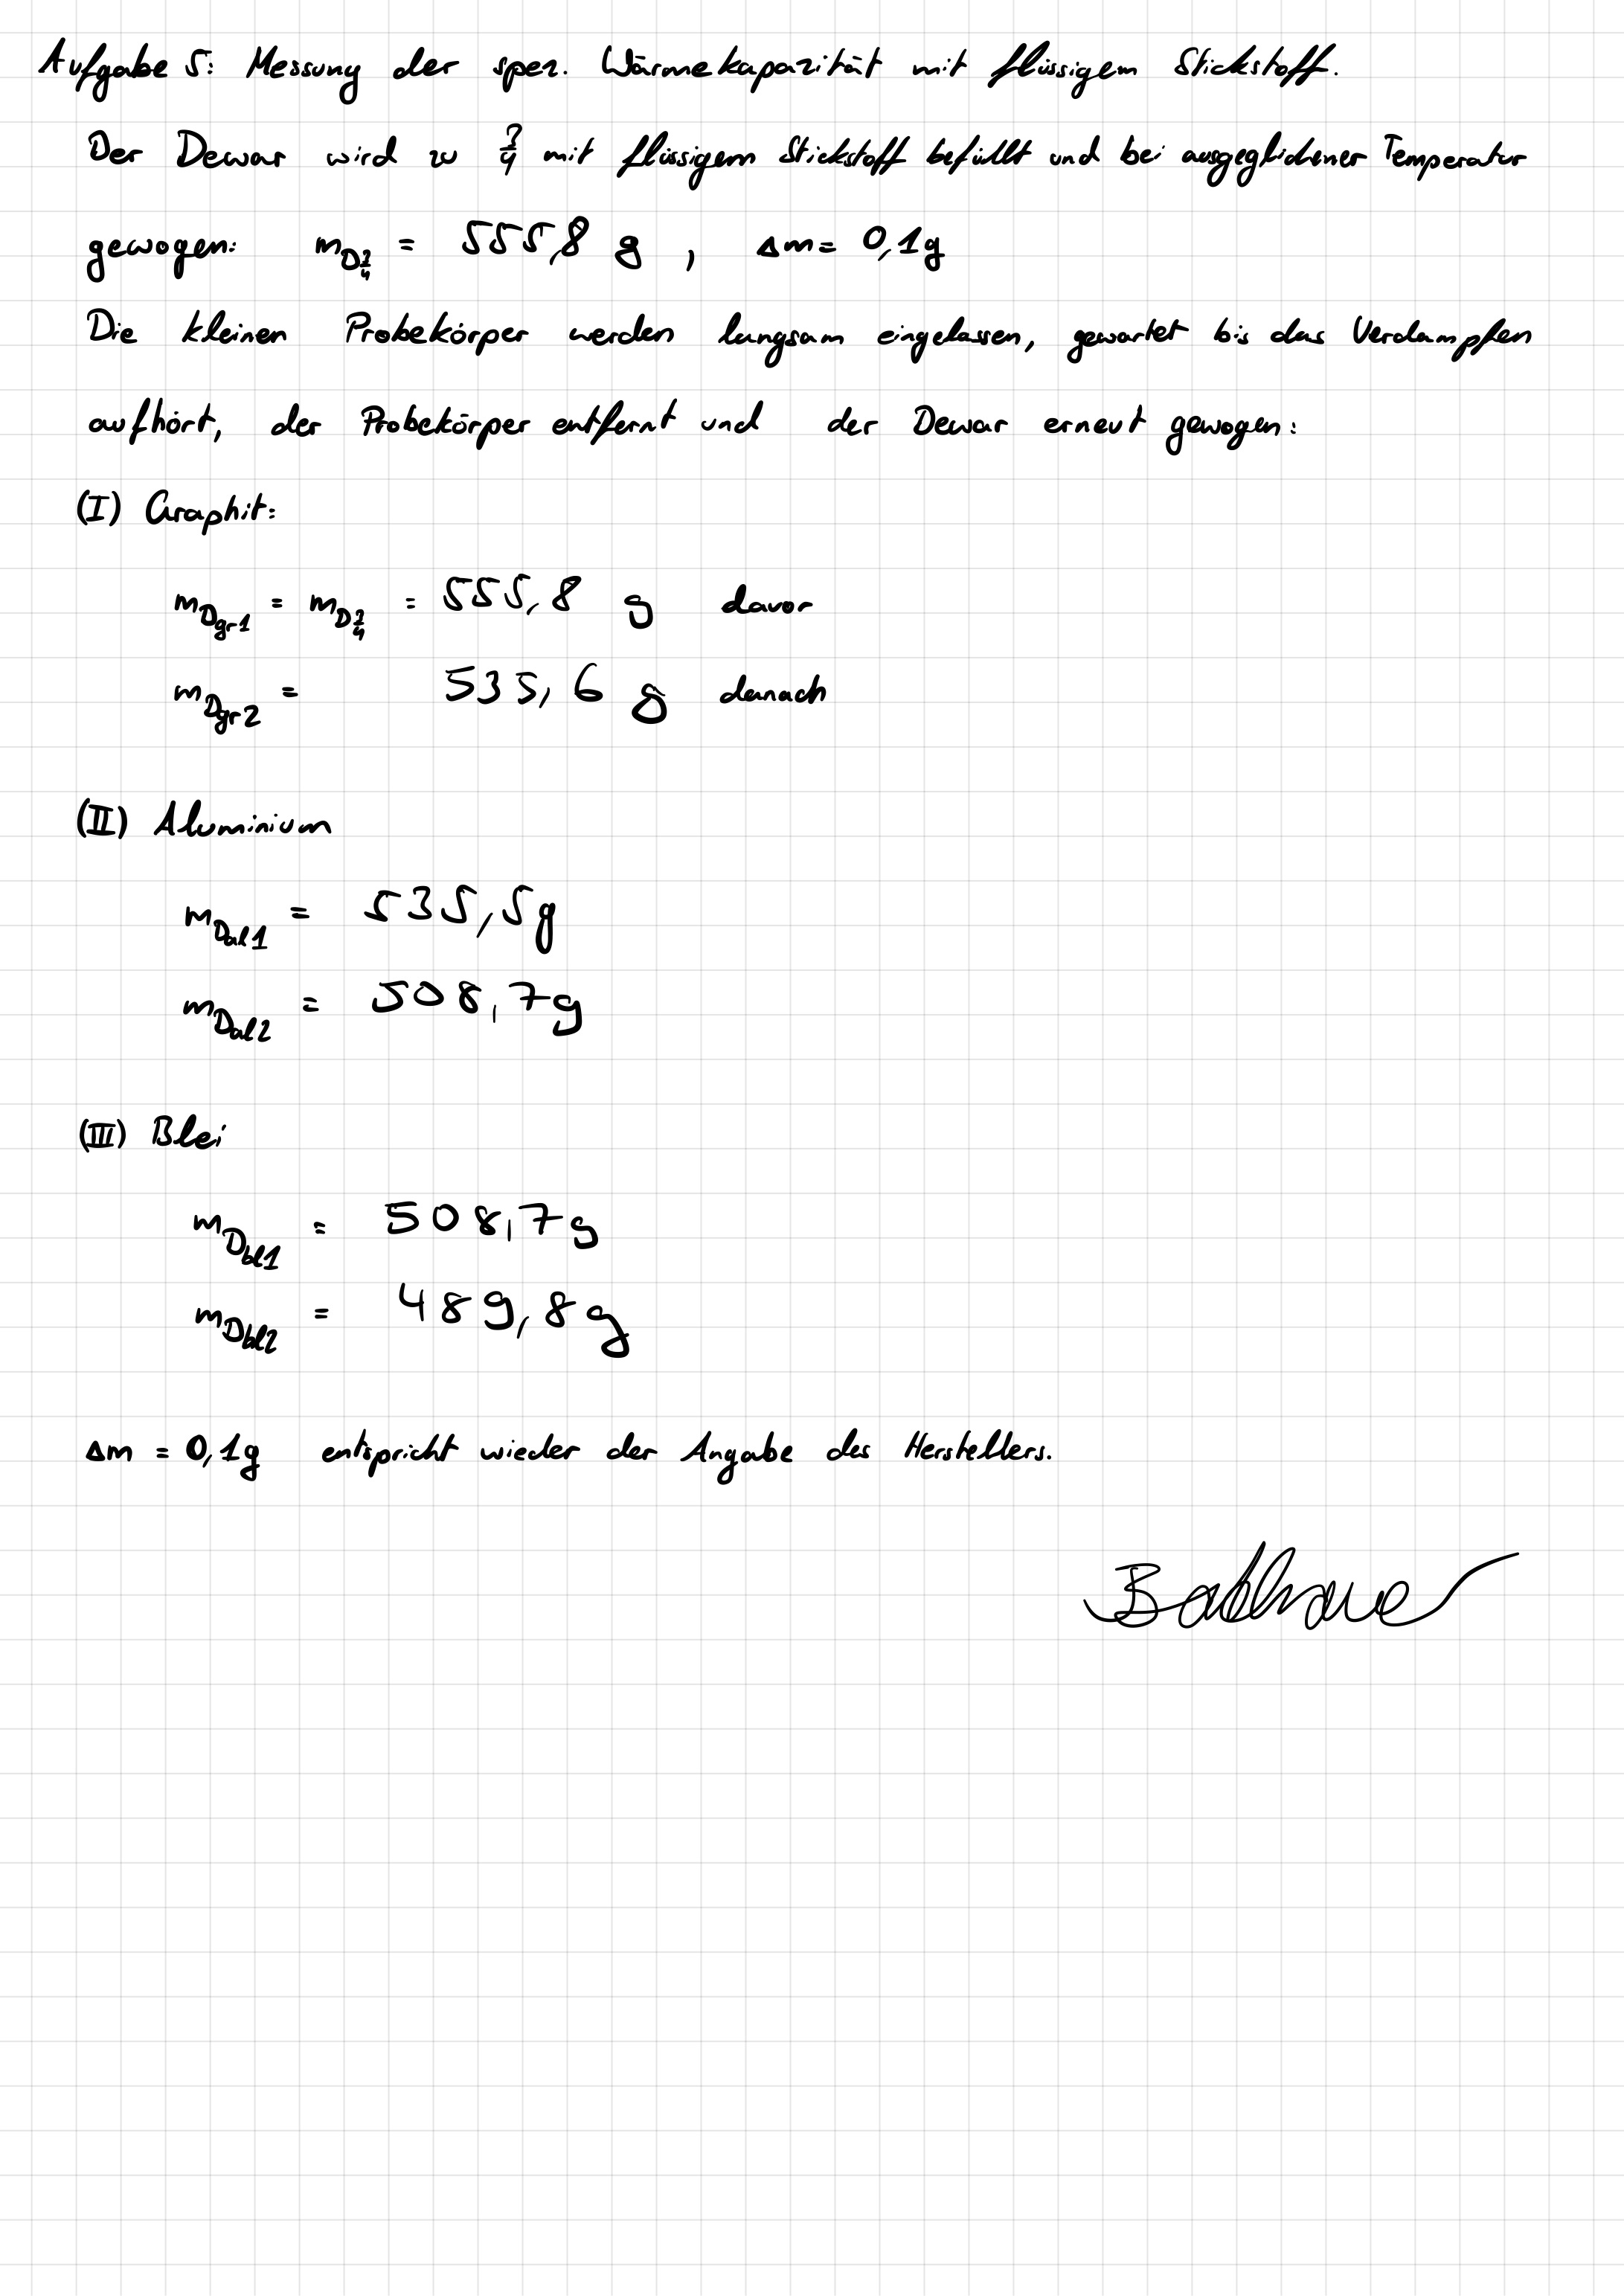
\includegraphics[width=\textwidth]{graphics/mess4.jpg}
\newpage

\addtocounter{table}{4}

%-------------------------AUSWERTUNG-------------------------
\section{Auswertung}

Zunächst werden alle Temperaturfehler des elektrischen Thermometers wie im Messprotokoll angegeben berechnet. Wir bekommen nach Rundungen auf die erste Nachkommastelle für alle Temperaturen aus Tabelle 1 einen Fehler von $\Delta T = 0,2^\circ$C und für alle aus den Tabellen 2 bis 4 einen Fehler von $\Delta T = 0,1^\circ$C.


\subsection{Bestimmung des Wasserwertes}

Zunächst soll mit den Messungen von Versuchsteil 3 der Wasserwert bestimmt werden. Dazu werden zunächst die Messungen von Tabelle 1 des Messprotokolls in ein Diagramm eingetragen, zu sehen in Abbildung 1. Hier ist noch zu erwähnen, dass wir uns bei der Messung etwas vertan und in der Tabelle einen Wert für $t=0$ gemessen haben, kurz nachdem wir das Kalorimeter befüllt hatten, wo eigentlich der vorher bestimmte Wert $T_1$ stehen sollte. Wir tragen im Diagramm also bei $t=0$ nicht den in der Tabelle notierten Wert von 54,9$^\circ$C ein, sondern 57,3$^\circ$C. Das ist im allgemeinen aber auch nicht so gravierend, da wir uns sowieso auf den linear abfallenden Teil der Messwerte fokussieren. Durch Extrapolation des linearen Teils kann nämlich die Mischungstemperatur $\overline{T}$ zum Zeitpunkt $t=0$ bestimmt werden und mit der Differenz zum Wert der Fehlergeraden der Fehler. Wir erhalten:

\begin{equation}
\begin{split}
    \overline{T} &= 54,55^\circ \text{C} \\
    \Delta \overline{T} &= | \overline{T} - \overline{T}_f | = 0,55^\circ \text{C} \\ \\
    \implies \bm{\overline{T}} &= \bm{(54,55 \pm 0,55)^\circ} \textbf{C}
\end{split}
\end{equation}

Wir bestimmen nun die Masse des Wassers über die Differenz der Massen des Kalorimeters mit und ohne Wasser sowie den Fehler per Fehlerfortpflanzung:

\begin{equation}
    \begin{split}
        m_w &= m_{K_1} - m_{K_0} = 238,50 \text{g} \\
        \Delta m_w &= \sqrt{(\Delta m_{K_1})^2 + (\Delta m_{K_0})^2} = 0,14 \text{g} \\ \\
        \implies \bm{m_w} &= \bm{(238,50 \pm 0,14)} \textbf{g}
    \end{split}
\end{equation}

Nun kann der Wasserwert $W$ bestimmt werden. Wir verwenden den Literaturwert $c_W = (4,186 \pm 0,004) \frac{\text{J}}{\text{g} \cdot \text{K}}$ aus dem Skript und berechnen den Fehler über Fehlerfortpflanzung:

\begin{equation}
    \begin{split}
        W &= m_W c_W \frac{T_1 - \overline{T}}{\overline{T} - T_2} = 94,8 \frac{\text{J}}{\text{K}} \\
        \Delta W &= m_W c_W \Biggl[ \left( \frac{1}{m_W} \frac{T_1 - \overline{T}}{\overline{T} - T_2} \cdot \Delta m_W \right)^2 + \left( \frac{1}{\overline{T} - T_2} \cdot \Delta T_1 \right)^2 \\
        &+ \left( \frac{T_1 - \overline{T}}{(\overline{T} - T_2)^2} \cdot \Delta T_2 \right)^2 + \left( \frac{T_1 - T_2}{(\overline{T} - T_2)^2} \cdot \Delta \overline{T} \right)^2 \\
        &+ \left( \frac{1}{c_W} \frac{T_1 - \overline{T}}{\overline{T} - T_2} \cdot \Delta c_W \right)^2 \Biggr]^{\frac{1}{2}} \\ \\
        &= m_W c_W \frac{T_1 - \overline{T}}{\overline{T} - T_2} \Biggl[ \left( \frac{1}{m_W} \cdot \Delta m_W \right)^2 + \left( \frac{1}{T_1 - \overline{T}} \cdot \Delta T_1 \right)^2 \\
        &+ \left( \frac{1}{\overline{T} - T_2} \cdot \Delta T_2 \right)^2 + \left( \frac{T_1 - T_2}{(\overline{T} - T_2)(T_1 - \overline{T})} \cdot \Delta \overline{T} \right)^2 \\
        &+ \left( \frac{1}{c_W} \cdot \Delta c_W \right)^2 \Biggr]^{\frac{1}{2}} \\
        &= 22,5\frac{\text{J}}{\text{K}} \\ \\
        \implies \bm{W} &= \bm{(94,8 \pm 22,5)} \frac{\textbf{J}}{\textbf{K}}
    \end{split}
\end{equation}

\begin{figure} [p]
    \centering
    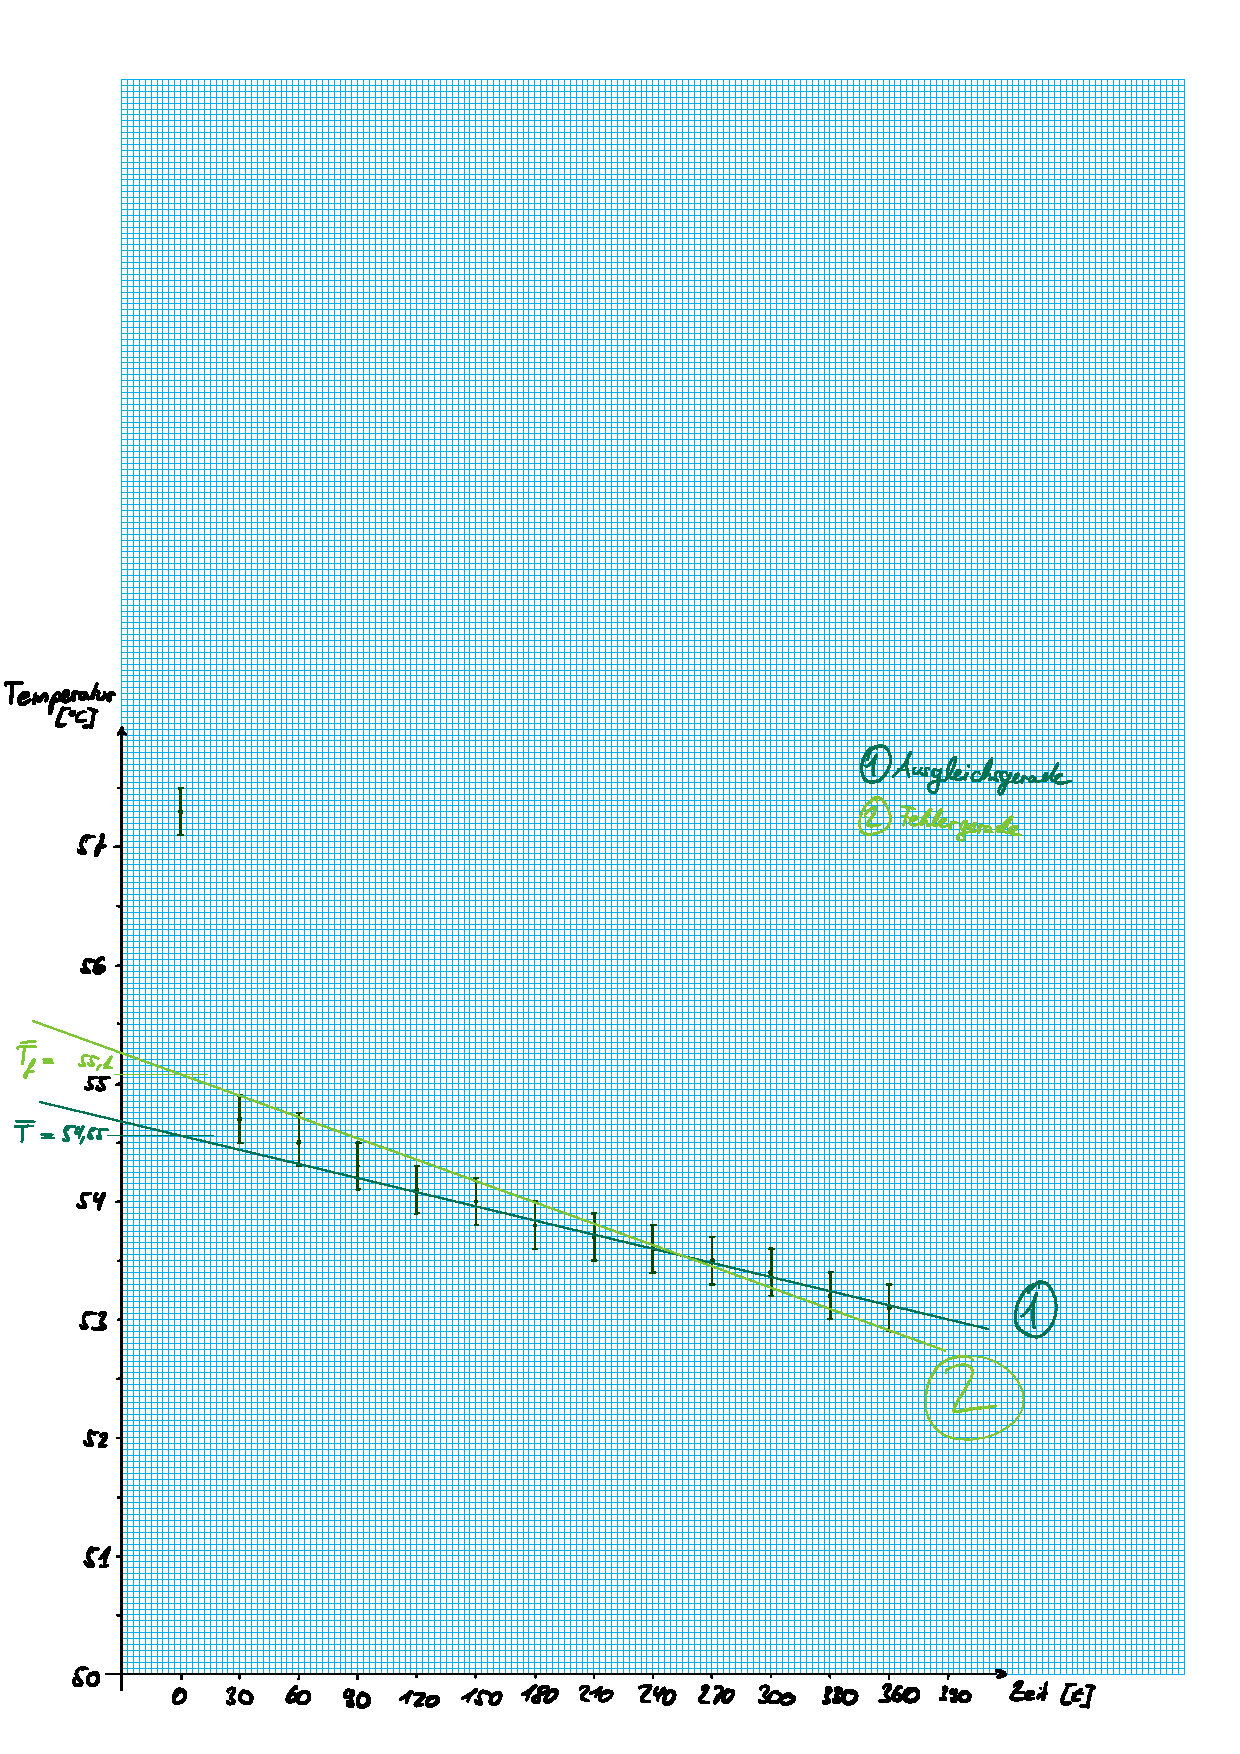
\includegraphics[width=\textwidth]{graphics/dia11.pdf}
    \caption{Bestimmung der Mischtemperatur $\overline{T}$}
\end{figure}


\newpage

\subsection{Bestimmung der Spezifischen Wäremkapazitäten und Molwärmen}

Zunächst bestimmen wir die Temperatur $T_1$ des kochenden Wassers aus dem Luftdruck sowie den Fehler über Fehlerfortpflanzung:

\begin{equation}
    \begin{split}
        T_1 &= 100^{\circ} \text{C} + 0,0276 \frac{^{\circ} \text{C}}{\text{hPa}} (p-1013 \text{hPa}) = 99,779^{\circ} \text{C} \\
        \Delta T_1 &= 0,0276 \frac{^{\circ} \text{C}}{\text{hPa}} \cdot \Delta p = 0,006^{\circ} \text{C}
    \end{split}
\end{equation}

Nun werden die Massen der Wassermengen bestimmt, bei denen die einzelnen Probekörper eingesetzt wurden. Dazu nimmt man erneut die Differenzen zwischen den Massen des gefüllten und leeren Kalorimeters und bestimmt den Fehler wieder über Fehlerfortpflanzung:

\begin{equation}
    \begin{split}
        m_{W_{gr}} &= m_{K_{gr}} - m_{K_0} = 308,50 \text{g} \\
        m_{W_{al}} &= m_{K_{al}} - m_{K_0} = 307,50 \text{g} \\
        m_{W_{bl}} &= m_{K_{bl}} - m_{K_0} = 307,30 \text{g} \\
        \Delta m_{W_{gr, al, bl}} &= \sqrt{(\Delta m)^2 + (\Delta m)^2} = 0,14 \text{g}
    \end{split}
\end{equation}

Aus den Messwerten lesen wir die Anfangstemperatur vom Wasserbad $T_2$ und die Mischungstemperatur $\overline{T}$ ab. Dabei entspricht $T_2$ der Temperatur die als letztes gemessen wurde, bevor der Probekörper eingelassen wurde, und $\overline{T}$ der Maximaltemperatur, die danach zu beobachten war. Der Fehler entspricht bei beiden Werten einfach dem Messfehler des Geräts. Wir bekommen somit:

\begin{equation}
    \begin{split}
        T_{2_{gr}} &= (24,4 \pm 0,1)^{\circ} \text{C} \\
        T_{2_{al}} &= (28,8 \pm 0,1)^{\circ} \text{C} \\
        T_{2_{bl}} &= (34,1 \pm 0,1)^{\circ} \text{C} \\ \\
        \overline{T}_{gr} &= (29,0 \pm 0,1)^{\circ} \text{C} \\
        \overline{T}_{al} &= (34,8 \pm 0,1)^{\circ} \text{C} \\
        \overline{T}_{bl} &= (37,3 \pm 0,1)^{\circ} \text{C} \\
    \end{split}
\end{equation}

Mit all diesen Werten können wir nun die spezifischen Wärmekapazitäten der drei Stoffe Graphit, Aluminium und Blei bestimmen. Wir verwenden Gleichung 4 sowie die entsprechenden Werte und erhalten:

\begin{equation}
    \begin{split}
        c_{gr} &= 0,72 \frac{\text{J}}{\text{g} \cdot \text{K}} \\
        c_{al} &= 0,82 \frac{\text{J}}{\text{g} \cdot \text{K}} \\
        c_{bl} &= 0,127 \frac{\text{J}}{\text{g} \cdot \text{K}} \\
    \end{split}
\end{equation}

Den Fehler bestimmen wir über Fehlerfortpflanzung und erhalten:

\begin{equation}
    \begin{split}
        \Delta c_x &= \Biggl[ \left( \frac{c_W (\overline{T} - T_2)}{m_x (T_1 - \overline{T})} \cdot \Delta m_W \right)^2 + \left( \frac{m_W (\overline{T} - T_2)}{m_x (T_1 - \overline{T})} \cdot \Delta c_W \right)^2 \\
        & + \left( \frac{(\overline{T} - T_2)}{m_x (T_1 - \overline{T})} \cdot \Delta W \right)^2 + \left( \frac{(c_W m_W + W) (T_1 - T_2)}{m_x (T_1 - \overline{T})^2} \cdot \Delta \overline{T} \right)^2 \\
        & + \left( \frac{(c_W m_W + W) (\overline{T} - T_2)}{m_x (T_1 - \overline{T})^2} \cdot \Delta T_1 \right)^2 + \left( \frac{c_W m_W + W}{m_x (T_1 - \overline{T})} \cdot \Delta T_2 \right)^2 \\
        & + \left( \frac{(c_W m_W + W) (\overline{T} - T_2)}{m_x^2 (T_1 - \overline{T})} \cdot \Delta m_x \right)^2 \Biggr] ^{\frac{1}{2}} \\ \\
        &= \frac{(\overline{T} - T_2)}{m_x (T_1 - \overline{T})} 
        \Biggl[ \left( c_W \cdot \Delta m_W \right)^2 + \left( m_W \cdot \Delta c_W \right)^2 + \left( \Delta W \right)^2 \\
        & + \left( \frac{(c_W m_W + W)(T_1-T_2)}{(T_1 - \overline{T})(\overline{T} - T_2)} \cdot \Delta \overline{T} \right)^2 + \left( \frac{c_W m_W + W}{T_1 - \overline{T}} \cdot \Delta T_1 \right)^2 \\
        & + \left( \frac{c_W m_W + W}{\overline{T} - T_2} \cdot \Delta T_2 \right)^2 + \left( \frac{c_W m_W + W}{m_x} \cdot \Delta m_x \right)^2 \Biggr]^{\frac{1}{2}} \\ \\
        \implies \Delta c_{gr} &= 0,08 \frac{\text{J}}{\text{g} \cdot \text{K}} \\
        \Delta c_{al} &= 0,10 \frac{\text{J}}{\text{g} \cdot \text{K}} \\
        \Delta c_{bl} &= 0,015 \frac{\text{J}}{\text{g} \cdot \text{K}} \\
    \end{split}
\end{equation}

\newpage
Die berechneten Werte der spezifischen Wärmekapazität der drei Stoffe ergeben sich also zu:

\begin{equation}
    \begin{split}
        \bm{c_{gr}} &= \bm{(0,72 \pm 0,08)} \frac{\textbf{J}}{\textbf{g} \cdot \textbf{K}} \\
        \bm{c_{al}} &= \bm{(0,82 \pm 0,10)} \frac{\textbf{J}}{\textbf{g} \cdot \textbf{K}} \\
        \bm{c_{bl}} &= \bm{(0,127 \pm 0,015)} \frac{\textbf{J}}{\textbf{g} \cdot \textbf{K}} \\
    \end{split}
\end{equation}

Wir vergleichen diese Werte mit den im Skript gegebenen Literaturwerten bei 300K, $c_{Pb} = 0,129 \frac{\text{J}}{\text{g} \cdot \text{K}}$, $c_{Al} = 0,90 \frac{\text{J}}{\text{g} \cdot \text{K}}$ und $c_{C} = 0,709 \frac{\text{J}}{\text{g} \cdot \text{K}}$:

\begin{equation}
    \begin{split}
        \sigma_{gr} &= \frac{|c_{gr} - c_{C}|}{\Delta c_{gr}} = 0,14 \\
        \sigma_{al} &= \frac{|c_{al} - c_{Al}|}{\Delta c_{al}} = 0,8  \\
        \sigma_{bl} &= \frac{|c_{bl} - c_{Pb}|}{\Delta c_{bl}} = 0,13 \\
    \end{split}
\end{equation}

Aus den Werten der spezifischen Wärmekapazität kann man, indem man die molare Masse $M$ multipliziert, die molare Wärmekapazität, auch Molwärme genannt, berechnen. Wir nutzen $M_{Pb} = 207,2 \frac{\text{g}}{\text{mol}}$, $M_{Al} = 26,98 \frac{\text{g}}{\text{mol}}$ und $M_{C} = 12,01 \frac{\text{g}}{\text{mol}}$ aus dem Skript und bekommen:

\begin{equation}
    \begin{split}
        c_{gr_m} &= c_{gr} M_{C} = 8,684 \frac{\text{J}}{\text{mol} \cdot \text{K}} \\
        c_{al_m} &= c_{al} M_{AL} = 22,1 \frac{\text{J}}{\text{mol} \cdot \text{K}} \\
        c_{bl_m} &= c_{bl} M_{Pb} = 26,30 \frac{\text{J}}{\text{mol} \cdot \text{K}} \\
    \end{split}
\end{equation}

Der Fehler wird über die Fehlerfortpflanzung berechnet:

\begin{equation}
    \begin{split}
        \Delta c_{x_m} &= M_X \cdot \Delta c_x \\ \\
        \implies \Delta c_{gr_m} &= 1,017 \frac{\text{J}}{\text{mol} \cdot \text{K}} \\
        \Delta c_{al_m} &= 2,7 \frac{\text{J}}{\text{mol} \cdot \text{K}} \\
        \Delta c_{bl_m} &= 3,06 \frac{\text{J}}{\text{mol} \cdot \text{K}} \\
    \end{split}
\end{equation}

Somit bekommen wir:

\begin{equation}
    \begin{split}
        \bm{c_{gr_m}} &= \bm{(8,684 \pm 1,017)} \frac{\textbf{J}}{\textbf{mol} \cdot \textbf{K}} \\
        \bm{c_{al_m}} &= \bm{(22,1 \pm 2,7)} \frac{\textbf{J}}{\textbf{mol} \cdot \textbf{K}} \\
        \bm{c_{bl_m}} &= \bm{(26,30 \pm 3,06)} \frac{\textbf{J}}{\textbf{mol} \cdot \textbf{K}} \\
    \end{split}
\end{equation}

Wir vergleichen diese Werte mit der theoretischen Aussage des Dulong-Petit-Gesetz, nachdem die Molwärme eines Festkörpers $C_V = 3R = 24,942 \frac{\text{J}}{\text{mol} \cdot \text{K}}$ beträgt, wobei $R$ die allgemeine Gaskonstante ist mit $R=8,314 \frac{\text{J}}{\text{mol} \cdot \text{K}}$ (Wikipedia, Stand: 17.09.2023). Im Vergleich bekommen wir:

\begin{equation}
    \begin{split}
        \sigma_{gr_m} &= \frac{|c_{gr_m} - C_V|}{\Delta c_{gr_m}} = 15,99 \\
        \sigma_{al_m} &= \frac{|c_{al_m} - C_V|}{\Delta c_{al_m}} = 1,05 \\
        \sigma_{bl_m} &= \frac{|c_{bl_m} - C_V|}{\Delta c_{bl_m}} = 0,44 \\
    \end{split}
\end{equation}

Wie man sieht sind bei Graphit signifikante Abweichungen zu erkennen.

\newpage
\subsection{Bestimmung der Wärmekapazitäten mit flüssigem Stickstoff}

Zur Bestimmung der Wärmekapazität im letzten Versuchsteil bestimmen wir zunächst die Differenzen zwischen den gemessenen Massen vor und nach dem Siedevorgang, um die verdampften Mengen Stickstoff $m_V$ zu bestimmen. Der Fehler der Differenzen setzt sich wie gewohnt aus zwei Messfehler zusammen zu $\Delta m_V = 0,14$g. Wir erhalten somit:

\begin{equation}
    \begin{split}
        m_{V_{gr}} &= (20,20 \pm 0,14) \text{g} \\
        m_{V_{al}} &= (26,80 \pm 0,14) \text{g} \\
        m_{V_{bl}} &= (18,90 \pm 0,14) \text{g} \\
    \end{split}
\end{equation}

Wir stellen Gleichung 5 um und identifizieren $T_1 = (25,6 \pm 1,6)^\circ$C als die Raumtemperatur und die der Probekörper,  $T_2 = -195,8^\circ$C als die Temperatur des Stickstoffs, $m_x$ als die Massen der kleinen Probekörper und $Q_V = 199 \frac{\text{J}}{\text{g}}$ als den gegebenen Literaturwert für die Verdampfungswärme von flüssigem Stickstoff. Wir berechnen so die spezifischen Wärmekapazitäten:

\begin{equation}
    \begin{split}
        c'_x &= \frac{m_V Q_V}{m_x (T_1 - T_2)} \\ \\
        \implies c'_{gr} &= 0,425 \frac{\text{J}}{\text{g} \cdot \text{K}} \\
        c'_{al} &= 0,723 \frac{\text{J}}{\text{g} \cdot \text{K}} \\
        c'_{bl} &= 0,1231 \frac{\text{J}}{\text{g} \cdot \text{K}} \\
    \end{split}
\end{equation}

Den Fehler berechnen wir über die Fehlerfortpflanzung:

\begin{equation}
    \begin{split}
        \Delta c'_x &= \frac{Q_V}{m_x (T_1 - T_2)} \Biggl[ \left( \Delta m_V \right)^2 + \left( \frac{m_V \Delta m_x}{m_x} \right)^2 + \left( \frac{m_V \Delta T_1}{T_1 - T_2} \right)^2 \Biggr]^{\frac{1}{2}} \\ \\
        \implies \Delta c'_{gr} &= 0,004 \frac{\text{J}}{\text{g} \cdot \text{K}} \\
        \Delta c'_{al} &= 0,007 \frac{\text{J}}{\text{g} \cdot \text{K}} \\
        \Delta c'_{bl} &= 0,0013 \frac{\text{J}}{\text{g} \cdot \text{K}} \\
    \end{split}
\end{equation}

Erneut bestimmen wir die Molwärme und deren Fehler:

\begin{equation}
    \begin{split}
        c'_{gr_m} &= c'_{gr} M_{C} = 5,10 \frac{\text{J}}{\text{mol} \cdot \text{K}} \\
        c'_{al_m} &= c'_{al} M_{AL} = 19,51 \frac{\text{J}}{\text{mol} \cdot \text{K}} \\
        c'_{bl_m} &= c'_{bl} M_{Pb} = 25,51 \frac{\text{J}}{\text{mol} \cdot \text{K}} \\ \\
        \Delta c'_{gr_m} &= M_{C} \cdot \Delta c'_{gr_m} = 0,05 \frac{\text{J}}{\text{mol} \cdot \text{K}} \\
        \Delta c'_{al_m} &= M_{Al} \cdot \Delta c'_{al_m} = 0,19 \frac{\text{J}}{\text{mol} \cdot \text{K}} \\
        \Delta c'_{bl_m} &= M_{Pb} \cdot \Delta c'_{pb_m} = 0,27 \frac{\text{J}}{\text{mol} \cdot \text{K}} \\ \\
        \implies \bm{c'_{gr_m}} &= \bm{(5,10 \pm 0,05)} \frac{\textbf{J}}{\textbf{mol} \cdot \textbf{K}} \\
        \bm{c'_{al_m}} &= \bm{(19,51 \pm 0,19)} \frac{\textbf{J}}{\textbf{mol} \cdot \textbf{K}} \\
        \bm{c'_{bl_m}} &= \bm{(25,51 \pm 0,27)} \frac{\textbf{J}}{\textbf{mol} \cdot \textbf{K}} \\
    \end{split}
\end{equation}

Es empfiehlt sich kurz klarzumachen, dass die hier berechneten $c'$ nicht 1:1 gleichzusetzen sind mit den im vorherigen Teil bestimmten $c$, sondern explizit die Wärmekapazitäten bei -195,8$^\circ$C sind, die im allgemeinen nicht gleich denen bei höheren Temperaturen sind. 

\newpage
Darauf basierend können wir das Verhältnis der spezifischen Molwärmen bei tiefer zu hoher Temperatur bestimmen. Wir erhalten:

\begin{equation}
    \begin{split}
        \frac{c'_{gr}}{c_{gr}} &= 0,59 \\
        \frac{c'_{al}}{c_{al}} &= 0,88 \\
        \frac{c'_{bl}}{c_{bl}} &= 0,97 \\
    \end{split}
\end{equation}

Und für den Fehler per Fehlerfortpflanzung:

\begin{equation}
    \begin{split}
        \Delta \frac{c'_{x}}{c_{x}} &= \frac{c'_{x}}{c_{x}} \sqrt{\left( \frac{\Delta c'_{x}}{c'_{x}} \right)^2 + \left( \frac{\Delta c_{x}}{c_{x}} \right)^2} \\ \\
        \Delta \frac{c'_{gr}}{c_{gr}} &= 0,07 \\
        \Delta \frac{c'_{al}}{c_{al}} &= 0,11 \\
        \Delta \frac{c'_{bl}}{c_{bl}} &= 0,11 \\
    \end{split}
\end{equation}

Somit bekommen wir:

\begin{equation}
    \begin{split}
        \bm{\frac{c'_{gr}}{c_{gr}}} &= \bm{0,59 \pm 0,07} \\
        \bm{\frac{c'_{al}}{c_{al}}} &= \bm{0,88 \pm 0,11} \\
        \bm{\frac{c'_{bl}}{c_{bl}}} &= \bm{0,97 \pm 0,11} \\
    \end{split}
\end{equation}

\newpage
Zuletzt nutzen wir das im Skript gegebene Diagramm im Anhang 3 und lesen an dem Grafen die Debey-Temperaturen mithilfe der berechneten Verhältnisse ab. Der Vorgang ist in Abbildung 2 zu sehen, der Fehler wurde großzügig abgeschätzt. Wir bekommen folgende Ergebnisse:

\begin{equation}
    \begin{split}
        \bm{T_{Debye_{gr}}} &= \bm{(750 \pm 25)} \textbf{K} \\
        \bm{T_{Debye_{al}}} &= \bm{(300 \pm 50)} \textbf{K} \\
        \bm{T_{Debye_{bl}}} &= \bm{(150 \pm 75)} \textbf{K} \\
    \end{split}
\end{equation}

\begin{figure} [!h]
    \centering
    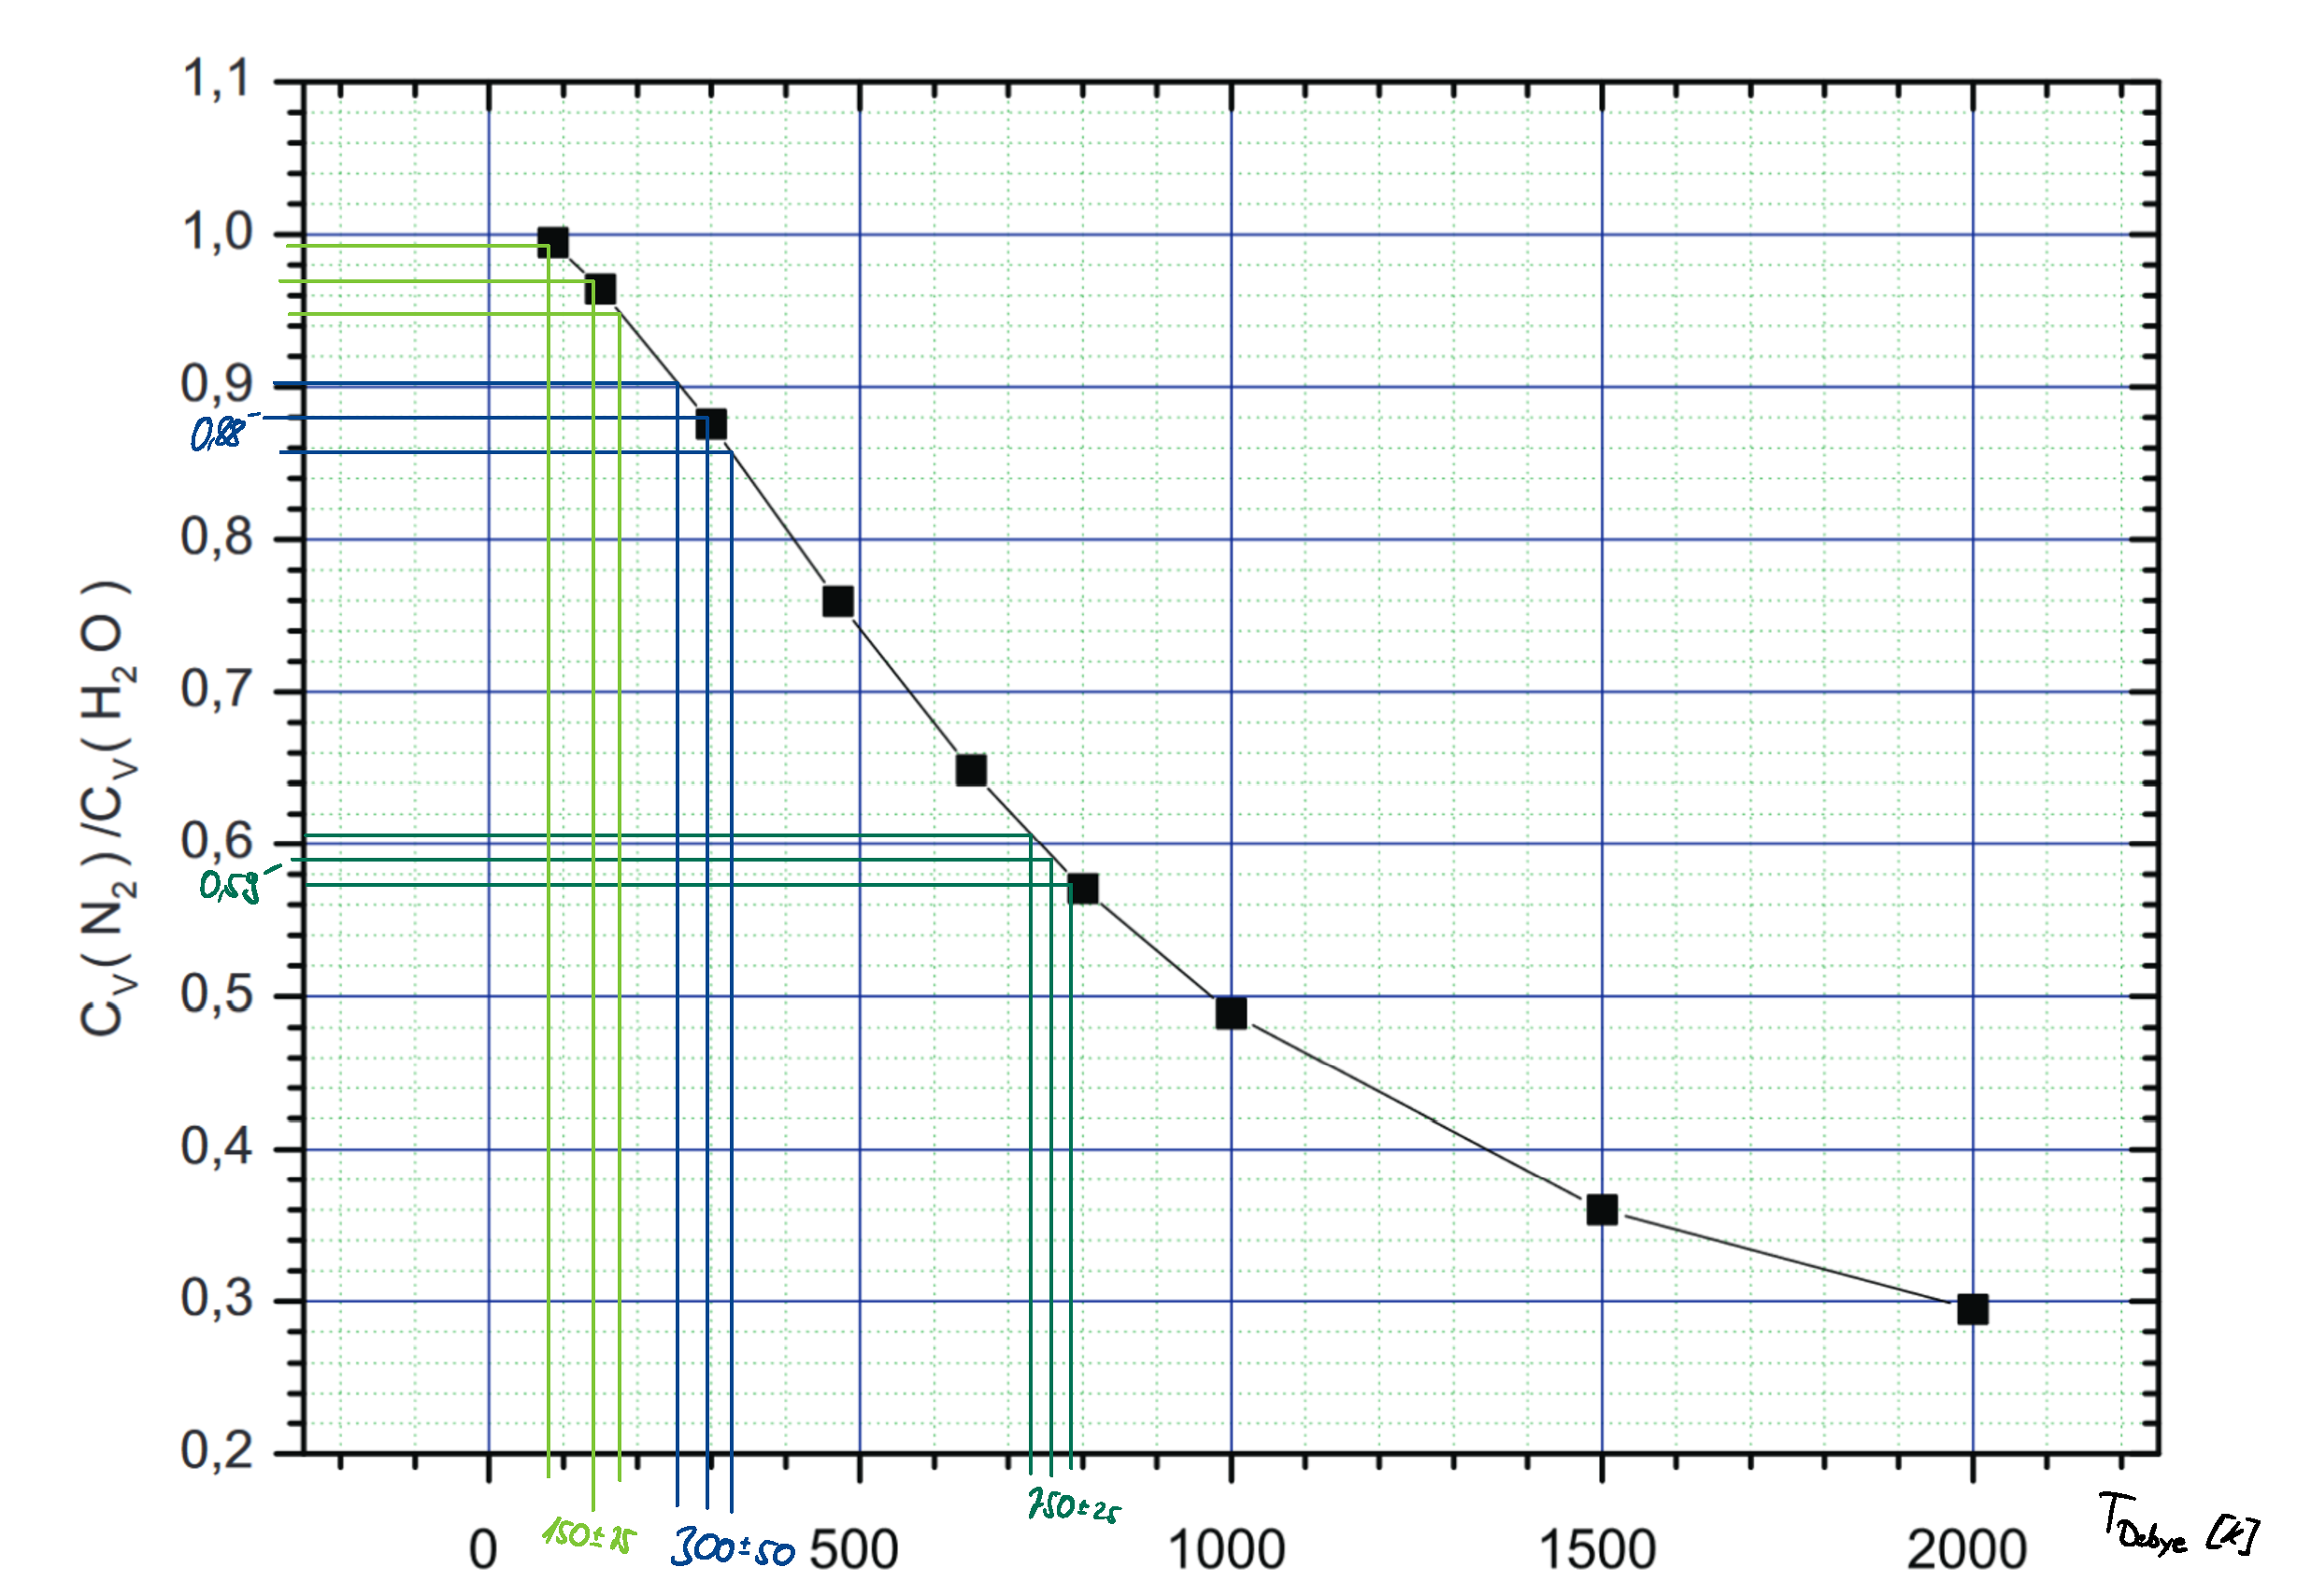
\includegraphics[width=\textwidth]{graphics/debye.pdf}
    \caption{Bestimmung der Debye-Temperatur}
\end{figure}

\newpage
%---------------PRÄSENTATION DER ENDERGEBNISSE---------------
\section{Präsentation der Endergebnisse}

In diesem Versuch wurde der Wasserwert des Kalorimeters bestimmt als 

\begin{equation}
    \bm{W} = \bm{(94,8 \pm 22,5)} \frac{\textbf{J}}{\textbf{K}}
\end{equation}

Daraufhin wurden die Spezifischen Wärmekapazitäten und Molwärmen drei verschiedener Materialien auf zwei verschiedene Weisen bestimmt. Über den Vergleich der beiden bestimmten Endwerte wurden die Debye-Temperaturen der Materialien bestimmt. Die Ergebnisse sind in folgender Tabelle aufgetragen. 

\begin{table}[!h]
    \centering
    \resizebox{\textwidth}{!}{
    \begin{tabular}{c|c|c|c|c|c}
        \textbf{Material} & $\bm{m}$ [g] & $\bm{c}$ $\left[ \frac{\text{J}}{\text{g} \cdot \text{K}} \right]$ &  $\bm{c_m}$ $\left[ \frac{\text{J}}{\text{mol} \cdot \text{K}} \right]$ & $\bm{\frac{c'_m}{c_m}}$ & $\bm{T_{Debye}}$ [K] \\ \hline
        Graphit & $124,6 \pm 0,1$ & $0,72 \pm 0,08$ & $8,684 \pm 1,017$ & $0,59 \pm 0,07$ & $750 \pm 25$ \\
        Aluminium & $155,7 \pm 0,1$ & $0,82 \pm 0,10$ & $22,1 \pm 2,7$ & $0,88 \pm 0,11$ & $300 \pm 50$ \\
        Blei & $557,3 \pm 0,1$ & $0,127 \pm 0,015$ & $26,30 \pm 3,06$ & $0,97 \pm 0,11$ & $150 \pm 75$ \\ \hline
        Graphit' & $42,7 \pm 0,1$ & $0,425 \pm 0,003$ & $5,10 \pm 0,04$ & - & - \\
        Aluminium' & $33,3 \pm 0,1$ & $0,723 \pm 0,004$ & $19,51 \pm 0,12$ & - & - \\
        Blei' & $138,0 \pm 0,1$ & $0,1231 \pm 0,0009$ & $25,51 \pm 0,19$ & - & - \\
    \end{tabular}}
    \caption{Zusammenfassung der relevanten Messgrößen für die Proben}
\end{table}

\newpage
%---------------ZUSAMMENFASSUNG UND DISKUSSION---------------
\section{Zusammenfassung und Diskussion}

In diesem Versuch wurden mit verschiedenen Messungen die Wärmekapazitäten verschiedener Körper untersucht. Indem zunächst der Wasserwert des Kalorimeters bestimmt wurde, konnten die Wärmekapazitäten von drei Materialien bestimmt werden, da der Temperaturverlauf aufgezeichnet wurde, als heiße Körper bestehend aus den Materialien in Wasser im Kalorimeter eingetaucht wurden. Hierbei wurde auch ein Vergleich mit der Theorie des Dulong-Petit-Gesetz erbracht. Ebenso konnten die Wärmekapazitäten ermittelt werden, indem man die Menge flüssigen Stickstoffs bestimmt, die beim Eintauchen der Probekörper verdampfte. Somit hatte man letztendlich zwei Werte der Molwärme, aus deren Quotient die Debye-Temperatur bestimmt werden konnte.

Zu den Versuchsergebnissen lässt sich zunächst sagen, dass alle Werte innerhalb erwarteter Bereiche und, sofern Literaturwerte gegeben waren, innerhalb insignifikanter Abweichungen vom Literaturwert blieben. Insbesonders die Ergebnisse der ersten berechneten spezifischen Wärmekapazitäten $c_x$ sind alle innerhalb der $1\sigma$-Umgebung des Literaturwerts und auch der Vergleich mit dem Dulong-Petit-Gesetz lieferte hier die erwarteten Ergebnisse, dass das Gesetz bei Materialien mit niedriger Debye-Temperatur, wie bei uns Blei, noch eher ungefähr der Realität entspricht als bei Materialien mit hoher Debye-Temperatur wie Graphit, wo starke Abweichungen bestimmt wurden. Bei der zweiten Reihe an bestimmten Wärmekapazitäten gab es zwar keine Vergleichswerte der Literatur, jedoch erscheinen die Ergebnisse im Vergleich miteinander sinnvoll und ergeben auch am Ende erwartete Ergebnisse bei den Quotienten und Debye-Temperaturen. 

Dennoch gibt es immer noch Aspekte bei sowohl der Durchführung als auch der Auswertung, bei denen potenzielle Fehlerquellen zu finden sind.

Zunächst lässt sich zum Experiment selbst die generelle Unsicherheit beim Arbeiten mit und Messen von Temperaturen nennen. Objekte auf die gewünschte Temperatur zu bringen ist nämlich immer etwas heikel, wie zum Beispiel das Erhitzen der Körper im Wasserbad sowie das darauffolgende Durchmischen der Temperaturen. Zum einen war der Prozess, bei dem man den heißen Körper ins Wasserbad brachte, schnell den Deckel schließen und den Timer starten musste sicherlich nicht optimal. Auch gab es keine Garantie, dass unsere Probekörper zu diesem Zeitpunkt schon lange genug im Wasserbad waren, um vollständig die Temperatur des kochenden Wassers anzunehmen, eine längere Wartezeit hätte hier eine größere Sicherheit gegeben, ist aber im Rahmen der eingeschränkten Zeit des Praktikums eventuell nur begrenzten realisierbar. Zum anderen haben wir während des Experimentierens gemerkt, dass unser Rührfisch des Magnetrührers häufiger mal gefühlt aus dem Gleichgewicht kam, was an einem Verstummen des typischen Reibungsgeräuschs zu höhren war, und dann erstmal wieder durch ein bisschen Hin- und Herbewegung des Drehknopfes zur Einstellung der RPM des Rührers in Bewegung versetzt werden musste. Da dies auch während Messungen mit Timer geschah, war hier währenddessen keine perfekte Durchmischung der Temperaturen garantiert. Bei genauerer Beobachtung schien dies an einer leichten Wölbung des Kalorimeterbodens nach oben in der Mitte der Fläche, wo dann genau der Rührfisch fixiert wird, zu liegen, die eventuell dafür sorgte, dass der Rührfisch bei seinen Umdrehungen nicht fest fixiert war und leicht nach außen abgelenkt werden konnte.

Bezüglich der Auswertung lässt sich generell noch die Ungenauigkeit des grafischen Verfahrens nennen. Manuell per Hand Punkte einzeichnen, Ausgleichsgeraden finden und Fehlergeraden abschätzen ist nämlich immer etwas ungenau. Insbesondere beim letzten Diagramm in Abbildung 2 war das finden der Debye-Temperaturen mit dem gegeben Diagram recht schwierig, da der gezeigte Graph vor allem bei den dicken Punkten schwer abzuschätzen war. Auch das Arbeiten und Ablesen beim ersten Diagramm sind von vornherein beim manuellen grafischen Verfahren fehlerbehaftet. Computerbasierte Visualisierungen hätten hier ein genaueres Ergebnis liefern können.

Zusammenfassend lässt sich sagen, dass sich trotz der genannten Fehlerquellen alle Ergebnisse des Versuchs innerhalb nachvollziehbarer Grenzen und erwarteten Beobachtungen einfanden und somit insgesamt zufriedenstellende Resultate erzielt wurden.

\end{document}



\begin{table}[!h]
    \centering
    \resizebox{\textwidth}{!}{
    \begin{tabular}{c|c|c|c|c|c|c}
        \textbf{Material} & $\bm{m_1}$ [g] & $\bm{m_2}$ [g] & $\bm{c_m}$ $\left[ \frac{\text{J}}{\text{mol} \cdot \text{K}} \right]$ & $\bm{c'_m}$ $\left[ \frac{\text{J}}{\text{mol} \cdot \text{K}} \right]$ & $\bm{\frac{c'_m}{c_m}}$ & $\bm{T_{Debye}}$ [K] \\ \hline
        Graphit & $42,7 \pm 0,1$ & $124,6 \pm 0,1$ & $8,684 \pm 1,017$ & $5,10 \pm 0,04$ & $0,59 \pm 0,07$ & $750 \pm 25$ \\
        Aluminium & $33,3 \pm 0,1$ & $155,7 \pm 0,1$ & $22,1 \pm 2,7$ & $19,51 \pm 0,12$ & $0,88 \pm 0,11$ & $300 \pm 50$ \\
        Blei & $138,0 \pm 0,1$ & $557,3 \pm 0,1$ & $26,30 \pm 3,06$ & $25,51 \pm 0,19$ & $0,97 \pm 0,11$ & $150 \pm 75$ \\
    \end{tabular}}
    \caption{Zusammenfassung der relevanten Messgrößen für die Proben}
\end{table}


\begin{table}[!ht]
    \centering
    \caption{Temperaturmessfehler Aufgabe 3}
    \begin{tabular}{c|c|c}
        \textbf{Zeit} $\bm{t}$ [s] & \textbf{Temperatur} $\bm{T}$ [$^\circ$C] & \textbf{Fehler} $\bm{\Delta T}$ [$^\circ$C] \\ \hline
        0 & 54,9 & 0,2 \\ 
        30 & 54,7 & 0,2 \\ 
        60 & 54,5 & 0,2 \\ 
        90 & 54,3 & 0,2 \\ 
        120 & 54,1 & 0,2 \\ 
        150 & 54 & 0,2 \\ 
        180 & 53,8 & 0,2 \\ 
        210 & 53,7 & 0,2 \\ 
        240 & 53,6 & 0,2 \\ 
        270 & 53,5 & 0,2 \\ 
        300 & 53,4 & 0,2 \\ 
        330 & 53,2 & 0,2 \\ 
        360 & 53,1 & 0,2 \\ 
    \end{tabular}
\end{table}

\begin{table}[!ht]
    \centering
    \caption{Temperaturmessfehler Aufgabe 4}
    \begin{tabular}{c|c|c|c}
        \textbf{Material} & \textbf{Zeit} $\bm{t}$ [s] & \textbf{Temperatur} $\bm{T}$ [$^\circ$C] & \textbf{Fehler} $\bm{\Delta T}$ [$^\circ$C] \\ \hline
        Graphit & 0 & 24,3 & 0,1 \\ 
        ~ & 60 & 24,2 & 0,1 \\ 
        ~ & 120 & 24,3 & 0,1 \\ 
        ~ & 180 & 24,3 & 0,1 \\ 
        ~ & 240 & 24,4 & 0,1 \\ 
        ~ & 300 & 24,4 & 0,1 \\ 
        ~ & 0 & 26,9 & 0,1 \\ 
        ~ & 10 & 28,5 & 0,1 \\ 
        ~ & 20 & 28,9 & 0,1 \\ 
        ~ & 30 & 29,0 & 0,1 \\ 
        ~ & 40 & 29,0 & 0,1 \\ 
        ~ & 50 & 29,0 & 0,1 \\ 
        ~ & 60 & 29,0 & 0,1 \\ 
        ~ & 70 & 29,0 & 0,1 \\ 
        ~ & 80 & 29,0 & 0,1 \\ 
        ~ & 90 & 29,0 & 0,1 \\ 
        ~ & 100 & 29,0 & 0,1 \\ 
        ~ & 110 & 29,0 & 0,1 \\ 
        ~ & 120 & 29,0 & 0,1 \\ 
        ~ & 130 & 29,0 & 0,1 \\ 
        ~ & 140 & 29,0 & 0,1 \\ 
        ~ & 150 & 28,9 & 0,1 \\ 
        ~ & 160 & 29,0 & 0,1 \\ 
        ~ & 170 & 28,9 & 0,1 \\ 
        ~ & 180 & 28,9 & 0,1 \\ 
        ~ & 190 & 29,0 & 0,1 \\ 
        ~ & 200 & 28,9 & 0,1 \\ 
        ~ & 210 & 29,0 & 0,1 \\ \hline
        Aluminium & 0 & 28,9 & 0,1 \\ 
        ~ & 60 & 28,8 & 0,1 \\ 
        ~ & 120 & 28,8 & 0,1 \\ 
        ~ & 180 & 28,8 & 0,1 \\ 
        ~ & 240 & 28,8 & 0,1 \\ 
        ~ & 300 & 28,8 & 0,1 \\ 
        ~ & 0 & 27,6 & 0,1 \\ 
        ~ & 10 & 33,9 & 0,1 \\ 
        ~ & 20 & 34,4 & 0,1 \\ 
        ~ & 30 & 34,6 & 0,1 \\ 
        ~ & 40 & 34,7 & 0,1 \\ 
        ~ & 50 & 34,8 & 0,1 \\ 
        ~ & 60 & 34,8 & 0,1 \\ 
        ~ & 70 & 34,8 & 0,1 \\ 
        ~ & 80 & 34,8 & 0,1 \\ 
        ~ & 90 & 34,7 & 0,1 \\ 
        ~ & 100 & 34,7 & 0,1 \\ 
        ~ & 110 & 34,7 & 0,1 \\ 
        ~ & 120 & 34,8 & 0,1 \\ 
        ~ & 130 & 34,7 & 0,1 \\ 
        ~ & 140 & 34,7 & 0,1 \\ 
        ~ & 150 & 34,7 & 0,1 \\ 
        ~ & 160 & 34,7 & 0,1 \\ 
        ~ & 170 & 34,7 & 0,1 \\ 
        ~ & 180 & 34,7 & 0,1 \\ 
        ~ & 190 & 34,7 & 0,1 \\ 
        ~ & 200 & 34,7 & 0,1 \\ 
        ~ & 210 & 34,6 & 0,1 \\ \hline
        Blei & 0 & 34,3 & 0,1 \\ 
        ~ & 60 & 34,3 & 0,1 \\ 
        ~ & 120 & 34,2 & 0,1 \\ 
        ~ & 180 & 34,2 & 0,1 \\ 
        ~ & 240 & 34,2 & 0,1 \\ 
        ~ & 300 & 34,1 & 0,1 \\ 
        ~ & 0 & 33,1 & 0,1 \\ 
        ~ & 10 & 36,4 & 0,1 \\ 
        ~ & 20 & 37,2 & 0,1 \\ 
        ~ & 30 & 37,3 & 0,1 \\ 
        ~ & 40 & 37,3 & 0,1 \\ 
        ~ & 50 & 37,3 & 0,1 \\ 
        ~ & 60 & 37,3 & 0,1 \\ 
        ~ & 70 & 37,3 & 0,1 \\ 
        ~ & 80 & 37,3 & 0,1 \\ 
        ~ & 90 & 37,3 & 0,1 \\ 
        ~ & 100 & 37,3 & 0,1 \\ 
        ~ & 110 & 37,3 & 0,1 \\ 
        ~ & 120 & 37,2 & 0,1 \\ 
        ~ & 130 & 37,3 & 0,1 \\ 
        ~ & 140 & 37,2 & 0,1 \\ 
        ~ & 150 & 37,2 & 0,1 \\ 
        ~ & 160 & 37,2 & 0,1 \\ 
        ~ & 170 & 37,2 & 0,1 \\ 
        ~ & 180 & 37,2 & 0,1 \\ 
        ~ & 190 & 37,2 & 0,1 \\ 
        ~ & 200 & 37,2 & 0,1 \\ 
        ~ & 210 & 37,1 & 0,1 \\ 
    \end{tabular}
\end{table}